\documentclass{mimosis}

\usepackage{metalogo}

%%%%%%%%%%%%%%%%%%%%%%%%%%%%%%%%%%%%%%%%%%%%%%%%%%%%%%%%%%%%%%%%%%%%%%%%
% Some of my favourite personal adjustments
%%%%%%%%%%%%%%%%%%%%%%%%%%%%%%%%%%%%%%%%%%%%%%%%%%%%%%%%%%%%%%%%%%%%%%%%
%
% These are the adjustments that I consider necessary for typesetting
% a nice thesis. However, they are *not* included in the template, as
% I do not want to force you to use them.

% This ensures that I am able to typeset bold font in table while still aligning the numbers
% correctly.
\usepackage{etoolbox}

%%%%%%%%%%%%%%%%%%%%%%%%%%%%%%%%%%%%%%%%%%%%%%%%%%%%%%%%%%%%%%%%%%%%%%%%
% Hyperlinks & bookmarks
%%%%%%%%%%%%%%%%%%%%%%%%%%%%%%%%%%%%%%%%%%%%%%%%%%%%%%%%%%%%%%%%%%%%%%%%

\usepackage[%
  colorlinks = true,
  citecolor  = RoyalBlue,
  linkcolor  = RoyalBlue,
  urlcolor   = RoyalBlue,
  unicode,
  ]{hyperref}

\usepackage{bookmark}

%%%%%%%%%%%%%%%%%%%%%%%%%%%%%%%%%%%%%%%%%%%%%%%%%%%%%%%%%%%%%%%%%%%%%%%%
% Bibliography
%%%%%%%%%%%%%%%%%%%%%%%%%%%%%%%%%%%%%%%%%%%%%%%%%%%%%%%%%%%%%%%%%%%%%%%%
%
% I like the bibliography to be extremely plain, showing only a numeric
% identifier and citing everything in simple brackets. The first names,
% if present, will be initialized. DOIs and URLs will be preserved.

\usepackage[%
  autocite     = plain,
  backend      = biber,
  doi          = true,
  url          = true,
  giveninits   = true,
  hyperref     = true,
  maxbibnames  = 99,
  maxcitenames = 99,
  sortcites    = true,
  style        = numeric,
  ]{biblatex}

\input{bibliography-mimosis}
\addbibresource{Thesis.bib}

\usepackage{wrapfig}
\usepackage[inline]{enumitem}
\setcapindent{0pt}
%%%%%%%%%%%%%%%%%%%%%%%%%%%%%%%%%%%%%%%%%%%%%%%%%%%%%%%%%%%%%%%%%%%%%%%%
% Fonts
%%%%%%%%%%%%%%%%%%%%%%%%%%%%%%%%%%%%%%%%%%%%%%%%%%%%%%%%%%%%%%%%%%%%%%%%

\ifxetexorluatex
  \usepackage{unicode-math}
  \setmainfont{EB Garamond}
  \setmathfont{Garamond Math}
  \setmonofont[Scale=MatchLowercase]{Source Code Pro}
\else
  \usepackage[lf]{ebgaramond}
  \usepackage[oldstyle,scale=0.7]{sourcecodepro}
  \singlespacing
\fi

% \newacronym[description={Principal component analysis}]{PCA}{PCA}{principal component analysis}
% \newacronym                                            {SNF}{SNF}{Smith normal form}
% \newacronym[description={Topological data analysis}]   {TDA}{TDA}{topological data analysis}

% \newglossaryentry{LaTeX}{%
%   name        = {\LaTeX},
%   description = {A document preparation system},
%   sort        = {LaTeX},
% }

% \newglossaryentry{Real numbers}{%
%   name        = {$\real$},
%   description = {The set of real numbers},
%   sort        = {Real numbers},
% }

\makeindex
\makeglossaries

%%%%%%%%%%%%%%%%%%%%%%%%%%%%%%%%%%%%%%%%%%%%%%%%%%%%%%%%%%%%%%%%%%%%%%%%
% Ordinals
%%%%%%%%%%%%%%%%%%%%%%%%%%%%%%%%%%%%%%%%%%%%%%%%%%%%%%%%%%%%%%%%%%%%%%%%

\makeatletter
\@ifundefined{st}{%
  \newcommand{\st}{\textsuperscript{\textup{st}}\xspace}
}{}
\@ifundefined{rd}{%
  \newcommand{\rd}{\textsuperscript{\textup{rd}}\xspace}
}{}
\@ifundefined{nd}{%
  \newcommand{\nd}{\textsuperscript{\textup{nd}}\xspace}
}{}
\makeatother

\renewcommand{\th}{\textsuperscript{\textup{th}}\xspace}

%%%%%%%%%%%%%%%%%%%%%%%%%%%%%%%%%%%%%%%%%%%%%%%%%%%%%%%%%%%%%%%%%%%%%%%%
% Incipit
%%%%%%%%%%%%%%%%%%%%%%%%%%%%%%%%%%%%%%%%%%%%%%%%%%%%%%%%%%%%%%%%%%%%%%%%

\title{Trajectory Control for High-DoF Manipulators}
\subtitle{In an environment filled with obstacles}
\author{Patrick Ondika}

\begin{document}

\frontmatter
  \begin{titlepage}
  \vspace*{5cm}
  \makeatletter
  \begin{center}
    \begin{Huge}
      \@title
    \end{Huge}\\[0.1cm]
    %
    \begin{Large}
      \@subtitle
    \end{Large}\\
    %
    \emph{by}\\
    \@author\\
    %
    \hfill
    \begin{figure}[h]
      \centering
      \includegraphics[width=0.4\textwidth]{fithesis-fi.pdf}
    \end{figure}

    \vfill
    \emph{Master's thesis}\\
    at\\
    \textsc{Masaryk University, Faculty of Computer Science}
  \end{center}
  \makeatother
\end{titlepage}

\newpage
\null
\thispagestyle{empty}
\newpage

  \begin{center}
  \textsc{Declaration}
\end{center}

\noindent

I hereby declare that this paper is my original authorial work, which
I have worked out on my own. All sources, references, and literature
used or excerpted during elaboration of this work are properly cited
and listed in complete reference to the due source.

\hspace*{\fill} Patrick Ondika

\newpage

\begin{center}
  \textsc{Acknowledgements}
\end{center}

\noindent

First and foremost, I'd like to thank Jan Mrázek, for creating the RoFI project, supporting me, and serving as a mentor. His encouragement and willingness to help have been very helpful throughout my entire time in the RoFI project. I'd also like to thank my advisor, Jiřík, for giving me feedback on my work and showing me that you can be successful without abandonning your inner 12-year old. The list goes on to all the other amazing people I met at the faculty; tutors and classmates that, often indirectly, gave me someone to look up to and the motivation to chase after them.

\newpage

\begin{center}
  \textsc{Abstract}
\end{center}
%
\noindent
%
RoFI is a platform of metamorphic robots -- robots consisting of individual modules which each work autonomously and have their own simple joints, but can connect to each other and complete more complex tasks. A natural shape for these robots to take is a robotic arm, which can manipulate with the surrounding objects. What separates RoFI arms from pre-built industrial arms is the total number of joints (degrees of freedom), which rises with each module.

An essential task for robotic arms (manipulators) is the act of moving one object from one place to the other. To successfully accomplish this task, we need to plan a trajectory the manipulator can take to reach the object, while avoiding collisions with potential obstacles. Various algorithms for this problem exist, but the complexity of standard methods scales exponentially with each degree of freedom, making them unusable for RoFI arms.

This thesis aims to design and implement an algorithm for trajectory planning of robotic manipulators with a very high degree of freedom. The thesis goes through the process of designing such an algorithm, explains the individual components, and presents the algorithm as a whole. Finally, the results are evaluated in a simulator within the RoFI environment.

\vfill
Keywords: RoFI, Metamorphic robots, Modular robots, Inverse kinematics, FABRIK, Motion planning, Path planning, Robotic manipulator


  \tableofcontents

\mainmatter

  % \part[A good part]{%
  %   A good part\\
  %   %
  %   \vspace{1cm}
  %   %
  %   \begin{minipage}[l]{\textwidth}
  %   %
  %   \textnormal{%
  %     \normalsize
  %     %
  %     \begin{singlespace*}
  %       \onehalfspacing
  %       %
  %       You can also use parts in order to partition your great work
  %       into larger `chunks'. This involves some manual adjustments in
  %       terms of the layout, though.
  %     \end{singlespace*}
  %   }
  %   \end{minipage}
  % }

  %%%%%%%%%%%%%%%%%%%%%%%%%%%%%%%%%%%%%%%%%%%%%%%%%%%%%%%%%%%%%%%%%%%%%%%%
\chapter{Introduction}
%%%%%%%%%%%%%%%%%%%%%%%%%%%%%%%%%%%%%%%%%%%%%%%%%%%%%%%%%%%%%%%%%%%%%%%%


In a world of automation, we would like to tell our robots a task such
as \enquote{Hand me a coffee.} and expect them to do it without giving
specific instructions of \textit{how} to do it.

This seemingly basic task contains many interesting subproblems, including but not limited to
the high level design of the robot, hardware design and programming, image or speech recognition, and human computer interaction.
For us, the critical part will be performing the task itself; in this case, computing and realising the movement necessary to grab a cup and deliver it to the target location.

A natural way for us to approach the problem is to create a humanoid robot, or simply a robotic arm on a fixed base. Even if we limit ourselves to the latter, the idea is quite fascinating; outside of making coffee for computer scientists, it can assist engineers or surgeons in their work.

This thesis aims to create a general algorithm for controlling robotic arms.
Our assumption is that we have a robotic arm that is fixed in place and has a high number of joints.
Naturally, the joints on the arm will have limited range, as many real arms do.
The task we are aiming to accomplish is to plan movement of the arm from one place to another, while avoiding collisions with other objects in the workspace of the arm.
The performed movement should be reasonably efficient, and the computation needs to be fast.

The presented methods will not be limited to a specific setup, but the results will be demostrated on top of the RoFI platform\cite{rofiPlatform}.

As computer scientists, we can already sense that we are tackling a rather complex problem, which is yet to be solved by the robotic community. Obstacles and joint constraints generally make the problem of motion planning\footnote{The general problem of computing the motion of a robot. It encompasses robotic arms as well as self driving cars and walking robots.} hard to perform, and the task of finding a good solution often goes directly against the task of finding a solution quickly.
There are many existing attempts to create an algorithm for motion planning of robotic arms,
some of which have been successfully used in practice to perform a specific task. Each method has specific advantages and disadvantages, which will be discussed in further chapters of this thesis.

What mostly sets our goals apart from previous research is the assumption that we have a high number of joints. This fact, at its core, makes traditional methods for related problems computationally infeasible.
Being unable to use a single existing method will lead us to decomposing the problem into smaller parts and combining various algorithms from different areas. By the end, we hope to build a satisfiable solution, starting with each component from the ground up.

Outside of robotics, having a general algorithm with this specification is interesting for computer graphics, in particular for generating character movement in videogames.
With an algorithm that can compute the motion of a constrained limb with a high number of joints at our disposal, we can design complex kinematic models and animate movement of the respective characters in complex environments.

%%%%%%%%%%%%%%%%%%%%%%%%%%%%%%%%%%%%%%%%%%%%%%%%%%%%%%%%%%%%%%%%%%%%%%%%
\section{Outline of the work}
%%%%%%%%%%%%%%%%%%%%%%%%%%%%%%%%%%%%%%%%%%%%%%%%%%%%%%%%%%%%%%%%%%%%%%%%

This thesis will try to lead the reader through the process of designing an algorithm for the motion planning of robotic arms. We will start with a more formal definition of the problem, preliminary knowledge, and introduction of the platform our solution will be presented on.

As we try to incrementally design an algorithm, the discussion of state of the art methods, some mathematical theory, and main ideas behind the implementation will be tied together to create the core of this thesis. Each idea will be accompanied by the intuition behind it, as well as a visual representation. Apart from the ideas that will build our final solution, we will explore methods that were not successful, and discuss the limits of different approaches.

Finally, the solution will be tested and evaluated. We will showcase the behavior of the algorithm in various environments, and present a possible application for it. We will run benchmarks to evaluate the efficiency and success rate of the algorithm. At the end, takeaways from the design process and further improvements will be discussed.

  \chapter{Preliminaries}

To start, we need to establish terminology and preliminary knowledge. Throughout this thesis, we will be discussing robotic arms; in robotic terms, they are more commonly referred to as \textit{manipulators}.

\begin{wrapfigure}{r}{0.25\textwidth}
    \centering
    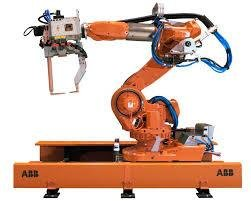
\includegraphics[width=0.35\textwidth]{Industrial-robotic-arm.jpeg}
  \caption{\\Industrial robotic arm with a gripper~\cite{manipulator}}
\end{wrapfigure}


Robotic manipulators are programmable mechanical devices, typically fixed in place. They are responsible for moving objects or tools and performing various tasks. They are widely used in factories for mass production of vehicles, electronics, etc. Based on the equipment of the specific manipulator, it can move objects from one assembly line to another, cut things, or solder parts together. However, such manipulators are often tailored to perform one specific motion repeatedly, thus, they will not be the focus of this work.

Manipulators consist of solid bodies, linked via movable joints. They often resemble human arms, although the specific shapes vary wildly.

We consider 2 basic types of joints, see Figure~\ref{fig:basicjoints}:
\begin{itemize}
  \item Revolute\footnote{Also referred to as rotary or rotational.} joints: the most common type. They consist of a motor rotating the next body around an axis. Depending on the type of motors and the build of the robot, the rotation may either be unbounded, or have a specific range of motion.
  \item Prismatic joints: these perform linear motion along the joint axis.
\end{itemize}

\begin{figure}[h]
\centering
\begin{subfigure}{.5\textwidth}
  \centering
  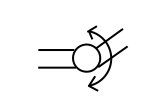
\includegraphics[width=.4\linewidth]{revolute.jpg}
  \caption{Revolute joints perform a rotation along their axis}
\end{subfigure}%
\begin{subfigure}{.5\textwidth}
  \centering
  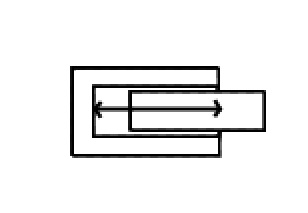
\includegraphics[width=.4\linewidth]{prismatic.png}
  \caption{Prismatic joints perform a linear motion along their axis}
\end{subfigure}
\caption{Basic joint types; the arrow refers to the respective range of motion.}
\label{fig:basicjoints}
\end{figure}

There are joint types that can perform more complicated motion, but they can generally be modelled as a combination of the basic two. Ball joints allow rotation in any direction; in a kinematic system, they can be modelled as two revolute joints in the same place. Cylindrical joints allow for both rotation and extension, serving as a combination of revolute and prismatic joints.

The state of the robot is called its configuration. A configuration is uniquely defined by two things:
\begin{itemize}
  \item The build of the robot: shape of the bodies, how they are connected, and the types of joints.
  \item The parameters of its joints.
\end{itemize}

The number of parameters that define a robotic system is referred to as degrees of freedom (DoF). Revolute and prismatic joints each have one degree of freedom. The parameter of a revolute joint is the current angle of rotation; the parameter of a prismatic joint is the current length it's extended at. Ball and cylindrical joints each have two degrees of freedom, respectively. The DoF of a robotic manipulator is the sum of DoFs of its flexible joints.

The end of a robotic arm is called the end effector. Typically, the end effector is different from the rest of the manipulator; it consists of a tool specialized to the robot's task. The end effector is designed to interact with the robot's environment, and there are many variatons. If the manipulator is designed to move objects, the end effector can be a fingerlike gripper, claw, or even use electromagnetic forces~\cite{grippers}. In handling textile materials, the end effector can be equipped with scissors, pins or needles.

When we refer to the position of the end effector, we mean its location and rotation in cartesian space. The parameter of a joint, such as its current rotation or extension, is sometimes called its position as well; not to be confused with its position in space. Though we will see that generally, knowing the joint parameters will let us compute their position in space, and vice versa.

\section{Kinematics of robotic manipulators}

The science that studies the relationship between joint parameters and the positions in cartesian space -- particularly the end effector -- is called kinematics.
We differentiate between forward and inverse kinematics.

Forward kinematics is the problem of finding the end effector position knowing the joint parameters. For manipulators with traditional joints, solving this problem is simple enough, and there is always a unique solution. The specifics differ based on the build of the robot, but there is a standard convention for it.

A method for computing forward kinematics was published by Denavit and Hartenberg in 1955~\cite{dh} and became the de-facto standard for robotics. The Denavit-Hartenberg (DH) method utilises $4\times4$ matrices to represent affine transformations in homogenous coordinates~\cite{nomizu1994affine}.
These matrices allow an efficient representation of both rotation and translation in 3D space.
In a kinematic system, such as a robot manipulator, each joint has its accompanying transformation matrix, and the position of the end effector is obtained by repeatedly applying the joint transformations through matrix multiplication. The base of the arm is commonly considered the origin of the manipulator's coordinate system, therefore it is simply the identity matrix:

\begin{equation}
  T_0 =  \begin{bmatrix}
            1 & 0 & 0 & 0 \\ 0 & 1 & 0 & 0 \\ 0 & 0 & 1 & 0 \\ 0 & 0 & 0 & 1 \\
          \end{bmatrix}
\end{equation}

Joint transformations are expressed as translations or rotations along the X and Z axes.
Translation along the Z axis is expressed as:

\begin{equation}
  Trans_Z(d) = \begin{bmatrix}
                 1 & 0 & 0 & 0 \\ 0 & 1 & 0 & 0 \\ 0 & 0 & 1 & d \\ 0 & 0 & 0 & 1 \\
               \end{bmatrix}
\end{equation}

Whereas the rotation is expressed as:

\begin{equation}
  Rot_Z(\theta) = \begin{bmatrix}
                    \cos{\theta} & -\sin{\theta} & 0 & 0 \\
                    \sin{\theta} & \cos{\theta} & 0 & 0 \\
                    0 & 0 & 1 & 0 \\ 0 & 0 & 0 & 1 \\
             \end{bmatrix}
\end{equation}

The transformations around the X axis are expressed analogously:

\begin{equation}
  Trans_X(r) = \begin{bmatrix}
                 1 & 0 & 0 & 0 \\ 0 & 1 & 0 & 0 \\ 0 & 0 & 1 & r \\ 0 & 0 & 0 & 1 \\
               \end{bmatrix}
\end{equation}


\begin{equation}
  Rot_X(\alpha) = \begin{bmatrix}
                    1 & 0 & 0 & 0 \\
                    0 & \cos{\alpha} & -\sin{\alpha} & 0 \\
                    0 & \sin{\alpha} & \cos{\alpha} & 0 \\
                    0 & 0 & 0 & 1 \\
             \end{bmatrix}
\end{equation}

Altogether, for a single joint i, we obtain the transformation matrix:

\begin{equation}
  T_i = \begin{bmatrix}
          \cos{\theta_i} & -\sin{\theta_i}\cos{\alpha_i} & \sin{\theta_i}\sin{\alpha_i} & r_i\cos{\theta_i} \\
          \sin{\theta_i} & \cos{\theta_i}\cos{\alpha_i} & -\cos{\theta_i}\sin{\alpha} & r_i\sin{\theta_i} \\
          0 & \sin{\alpha_i} & \cos{\alpha_i} & d_i \\
          0 & 0 & 0 & 1 \\
        \end{bmatrix}
\end{equation}

To obtain the position of the end effector (or any other link) of a manipulator, we simply need to multiply all the joint transformations leading up to it:

\begin{equation}
  [T] = T_0T_1\cdots T_{n-1}T_n
\end{equation}

Notice that each matrix in the Denavit-Hartenberg convention is in form
\[
    T = \begin{bmatrix}
        \begin{array}{c|c}
           \begin{matrix}
              & & & \\
              & & R & & \\
              & & &
           \end{matrix}
            & t \\
        \midrule
        \begin{matrix}
              0 & 0 & 0 \\
           \end{matrix}
            & 1 \\
        \end{array}
    \end{bmatrix}
\]
\noindent where R is the $3\times3$ rotational part of the matrix, which is always orthonormal, and $t$ represents the displacement along the 3 axes. This allows for efficient computation of the inverse, since the inverse of an orthonormal matrix is equal to its transpose, and the inverse of a translation is simply its negation. By multiplying the two inversions, we get:

\[
    T^{-1} = \begin{bmatrix}
        \begin{array}{c|c}
           \begin{matrix}
              & & & \\
              & & R^T & & \\
              & & &
           \end{matrix}
            & -R^{T}t \\
        \midrule
        \begin{matrix}
              0 & 0 & 0 \\
           \end{matrix}
            & 1 \\
        \end{array}
    \end{bmatrix}
\]

Knowing the transformation matrix of a specific joint allows us to easily compute the positions of joints. Knowing the inverse of a joint's transformation matrix allows us to easily compute positions of other objects in the workspace with respect to the joint, which will be useful later on.

Since the movements of traditional joints can easily be represented as a combination of the two rotations and translations, we consider the forward kinematics of robotic manipulators a solved problem.

\newpage

\begin{wrapfigure}{r}{0.25\textwidth}
    \centering
    \begin{minipage}{.25\textwidth}
        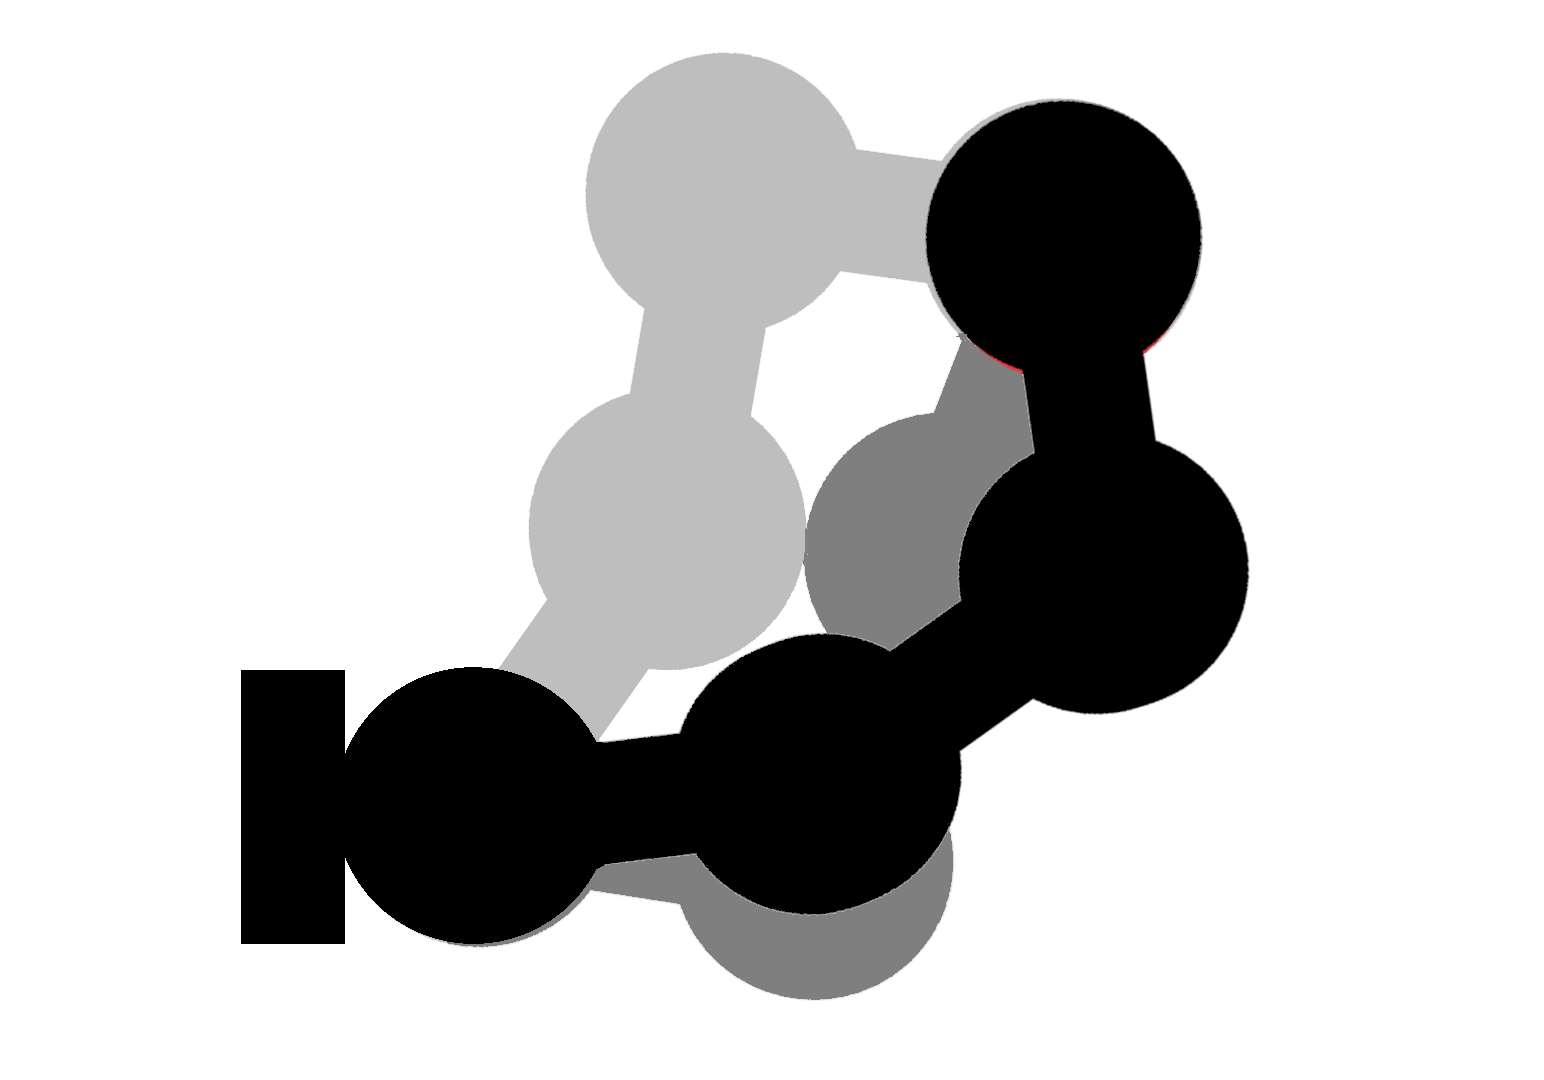
\includegraphics[width=\textwidth]{redundant.png}
    \end{minipage}
    \caption{\\3 example IK solutions to the same problem~\cite{Ondika2021thesis}}\label{fig:redun}
\end{wrapfigure}

Inverse kinematics (IK), as the name suggests, is the inverse to the forward kinematics problem: given a position for the end effector, we wish to compute the corresponding joint parameters. This is a significantly harder problem. If there are exactly as many degrees of freedom in the manipulator as the dimension of the target\footnote{Industrial manipulators commonly have exactly 6 degrees of freedom, which corresponds to a target in cartesian space, consisting of the x-y-z dimensions and a rotation around each of the axes.}, there are ways to obtain an exact analytical solution. However, as we are considering manipulators with a significantly higher DoF, there will generally be an infinite number of solutions (see Figure~\ref{fig:redun}). Hence, numerical methods have to be used.

Common methods for solving inverse kinematics view the problem as an optimization problem, and iteratively try to minimize the distance between the target and the current position of the end effector. All the different methods for inverse kinematics are not the topic of this thesis, and only a short summary will be provided. For a complete overview, see~\cite{overview}.

The methods most discussed in literature are based on approximating the inversion of a Jacobian matrix. For robotic manipulators, the Jacobian matrix is a matrix of partial derivatives at each joint. The size of the matrix is $m \times n$, where $m$ corresponds to the target dimension (6 for the 3D problem of reaching a target) and $n$ corresponds to the degrees of freedom.
The Jacobian matrix provides us with a linear approximation of how the end effector is going to move when slight changes in the joint positions are made. Hence, if we could invert this matrix, we would get an estimation of how to move the joints in order to move the end effector closer to the target. Then, by iteratively repeating this process, we could obtain a solution. However, the Jacobian matrix generally does not have an inversion; the matrix is not square for manipulators with over 6 degrees of freedom, and even then, the determinant is not guaranteed to be nonzero.

There are many methods that try to approximate the inverse, most notably the Moore-Penrose inverse, known as the matrix pseudoinverse~\cite{penrose_1955}. This matrix serves as the generalisation of the matrix inverse, and exists for any matrix. The Jacobian pseudoinverse technique for inverse kinematics was heavily studied, but it suffers from a few fundamental drawbacks. It's hard to incorporate local joint limits, and the method behaves erratically near singularities -- a state where the manipulator is straightened out and slight movement of any joint results in roughly the same change.
In addition to that, it is not very efficient, as the Jacobian matrix and its pseudoinverse have to be computed repeatedly in each iteration. A common way to compute the pseudoinverse is using Singular Value Decomposition; the complexity of this method is $\mathcal{O}(mn^2)$~\cite{trefethen1997numerical}, which scales poorly with respect to the degrees of freedom.

Some authors~\cite{Wolovich1984ACT} suggest using the transpose of the Jacobian matrix, rather than the pseudoinverse. This method is faster but less precise, and suffers from many of the same problems. There are many modifications and extensions of these algorithms, but since we are considering high-DoF manipulators, they are not as interesting for us.

The other branch of inverse kinematics algorithms are heuristic techniques. These consist of simpler computations and make decisions locally at each joint. They are faster, scale linearly with respect to the DoF of the manipulator and can easily be extended with joint limits. However, due to making local decisions, these methods can struggle with computing collision free positions or providing any other guarantees about the resulting position of the arm.

\begin{wrapfigure}{r}{0.35\textwidth}
    \centering
    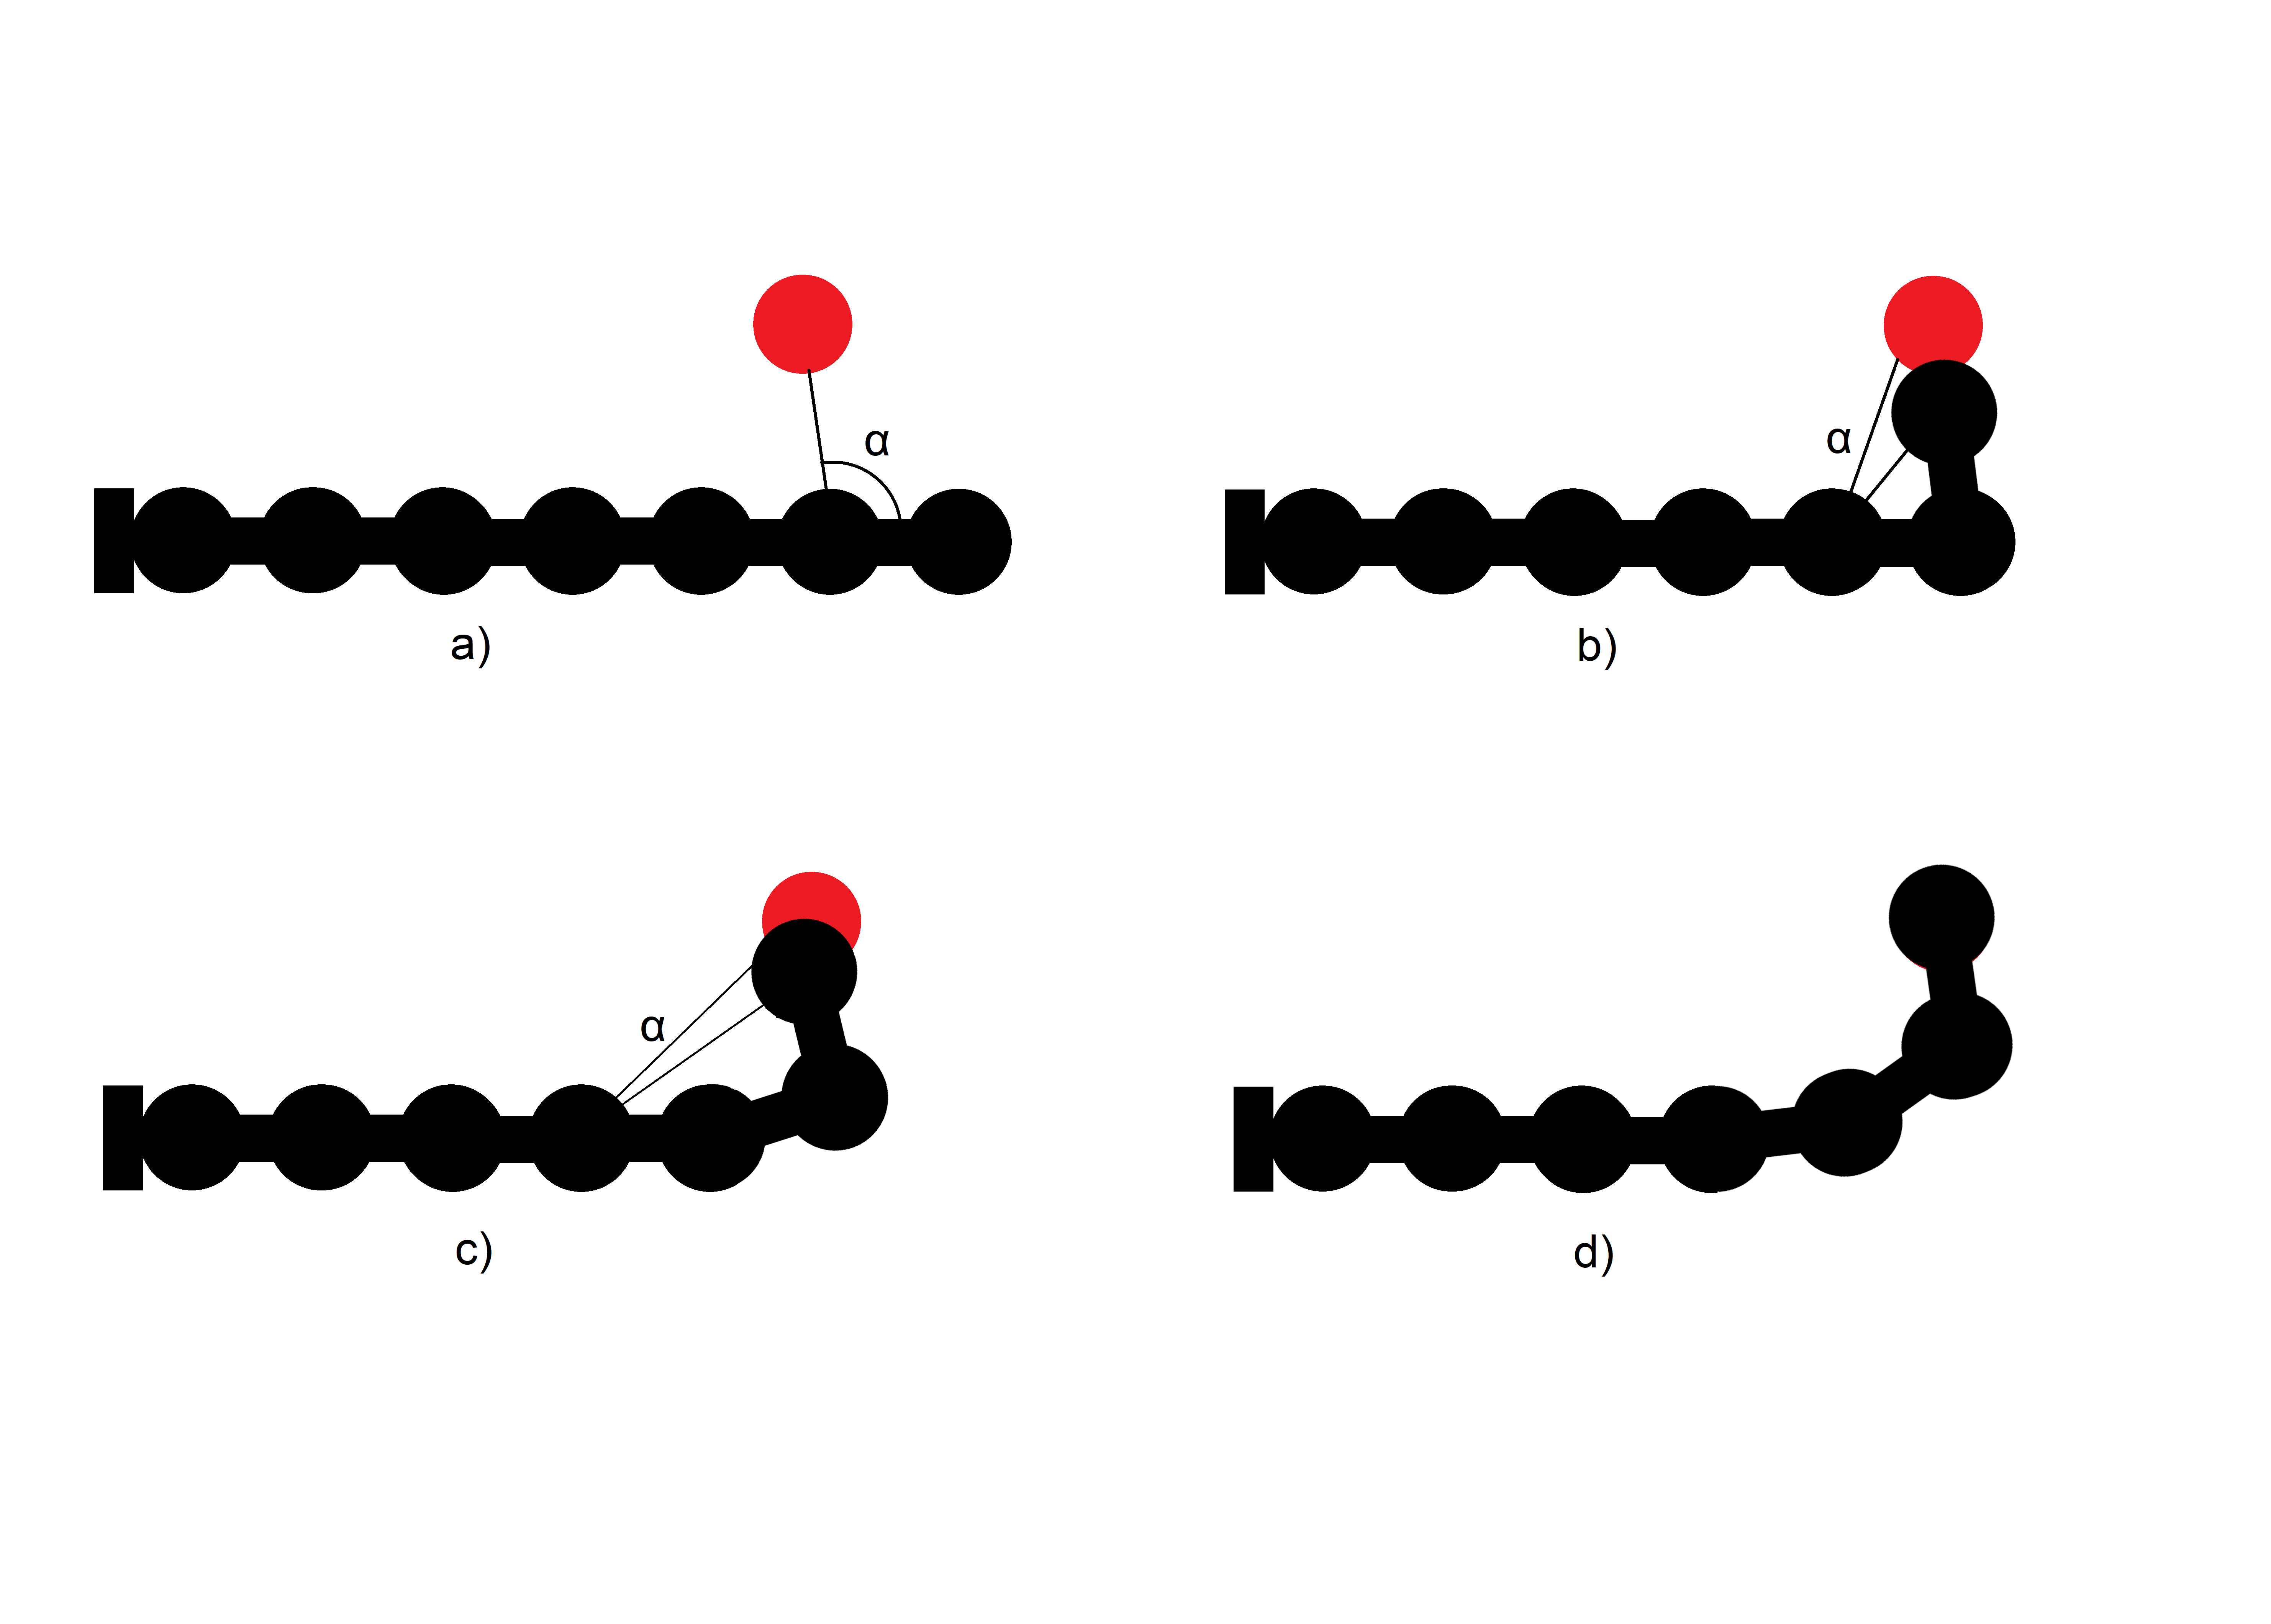
\includegraphics[width=0.35\textwidth]{ccd1.png}
    \caption{\\CCD algorithm~\cite{Ondika2021thesis}: The angles are repeatedly computed for each joint until a solution is found}
    \label{fig:ccd}
\end{wrapfigure}

The simplest of these methods is Cyclic Coordinate Descent (CCD)~\cite{ccd}. This algorithm iteratively goes through the joints of the manipulator, starting at the end effector, and turns each of them so that the distance to the target is locally minimized. Once it reaches the base, it starts iterating from the end again, until the end effector is close enough to the target (see Figure~\ref{fig:ccd}). This algorithm is fast, scales well, and in an unconstrained system, it always finds a solution, if one exists. However, the reached positions are very unnatural, which can lead to collisions with the environment, or even the manipulator itself. If we add obstacles or joint limits, the algorithm is also susceptible to local minima.

The state of the art method for inverse kinematics is the heuristic algorithm FABRIK:\ Forward and Backward Reaching Inverse Kinematics~\cite{fabrik}.
The algorithm consists of simple geometric computations, which are very fast. Just like the CCD method, it always finds a solution in unconstrained systems, and scales very well. Unlike CCD, it converges significantly quicker and computes natural poses.

\begin{figure}
    \centering
    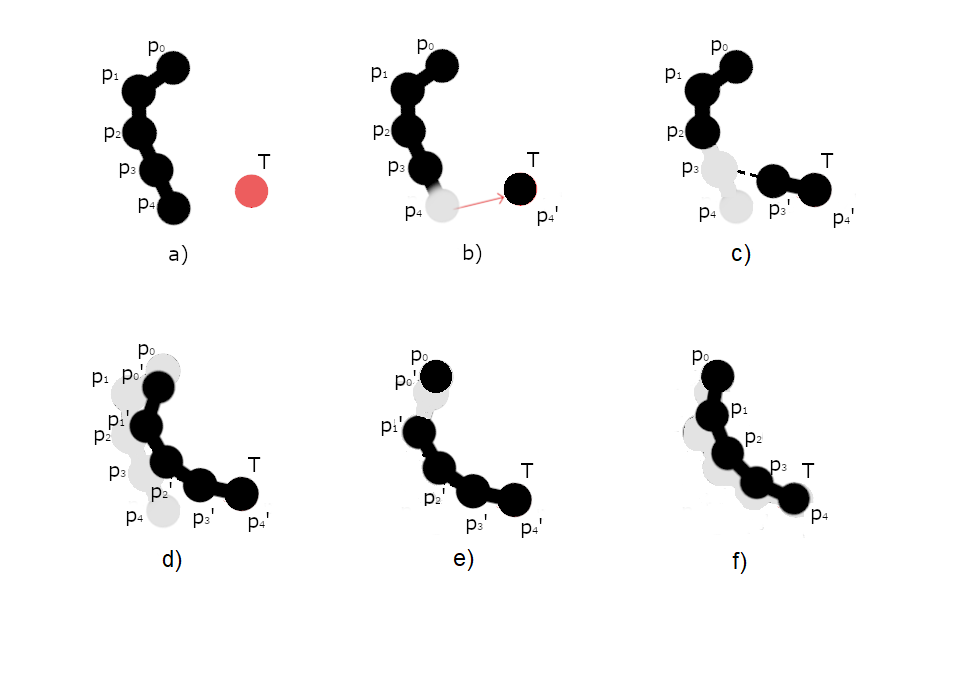
\includegraphics[width=0.8\textwidth]{fabrik.png}
    \caption[]{Fabrik algorithm~\cite{Ondika2021thesis}:
      \begin{enumerate*}
        \item[(a)] the initial position of the arm and the target
        \item[(b)] the end-effector $p_4$ is moved to the desired position
        \item[(c)] a vector between $p_3$ and the new $p_4$ is found, $p_3$ is repositioned along this line
        \item[(d)] arm after the forward reaching stage
        \item[(e)] the first point is moved to its initial position; the algorithm repeats itself in the other direction
        \item[(f)] final state; the base is in place and the target has been reached
       \end{enumerate*}
    }
    \label{fig:fab}
  \end{figure}

Rather than working with matrices or joint angles, the basic version of the algorithm calculates with points. As the name suggests, each iteration of the algorithm consists of two stages. In the first, forward reaching stage, the end-effector is moved to the desired target. Then, for each joint, the algorithm computes a line between the current and the next joint, which has already been moved. The current joint is moved along this line to the original distance between the two joints. Afterwards, the process is repeated for every joint, up until the base.

At this point, the algorithm has reached the target, but the immovable base may have been assigned a new position. Hence the algorithm is repeated, but this time it sets the base to the initial position and follows through with the algorithm all the way to the top. This forward and backward reaching is repeated until the base remains in its initial position and the end-effector reaches the target. Figure~\ref{fig:fab} illustrates the procedure.

The basic version of the algorithm is presented with rotational joints, but can be extended to any of the common types~\cite{fabrikConstraints}.

The FABRIK algorithm is very powerful and will serve us further, but note that inverse kinematics is just a subproblem of robot manipulator control. Even if we are able to compute the desired joint parameters for reaching a target, it remains unclear how to perform the motion from the initial position to the computed one. If there are obstacles in the environment, simply moving the joints to the computed positions is not possible.

\begin{figure}
\centering
\begin{subfigure}{.3\textwidth}
  \centering
  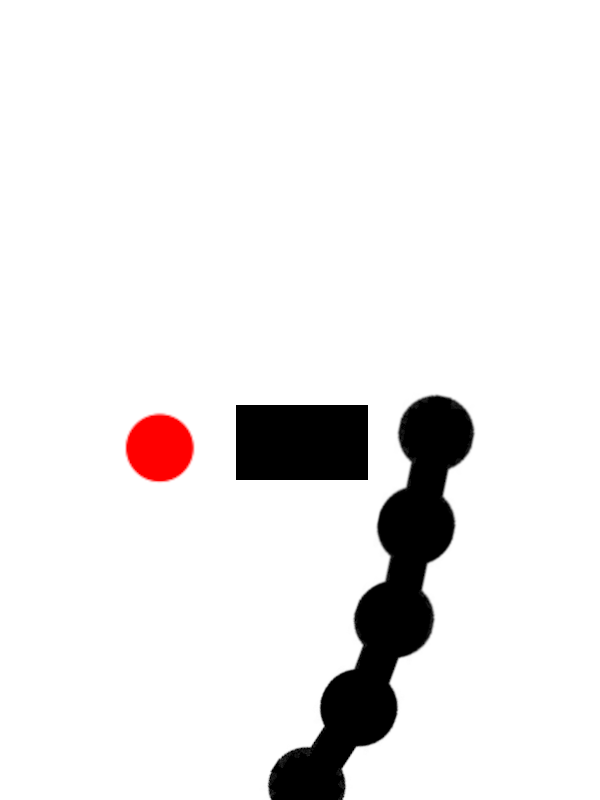
\includegraphics{IK_target.png}
  \caption{Initial position of the manipulator, a rigid obstacle and a target}
\end{subfigure}%
\begin{subfigure}{.3\textwidth}
  \centering
  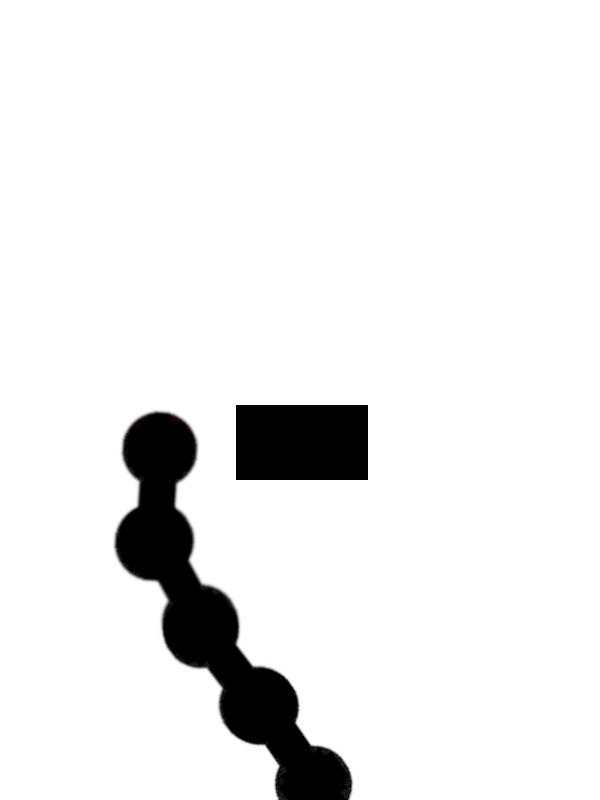
\includegraphics{IK_solution.png}
  \caption{A valid solution where the target is reached by the end effector}
\end{subfigure}%
\begin{subfigure}{.3\textwidth}
  \centering
  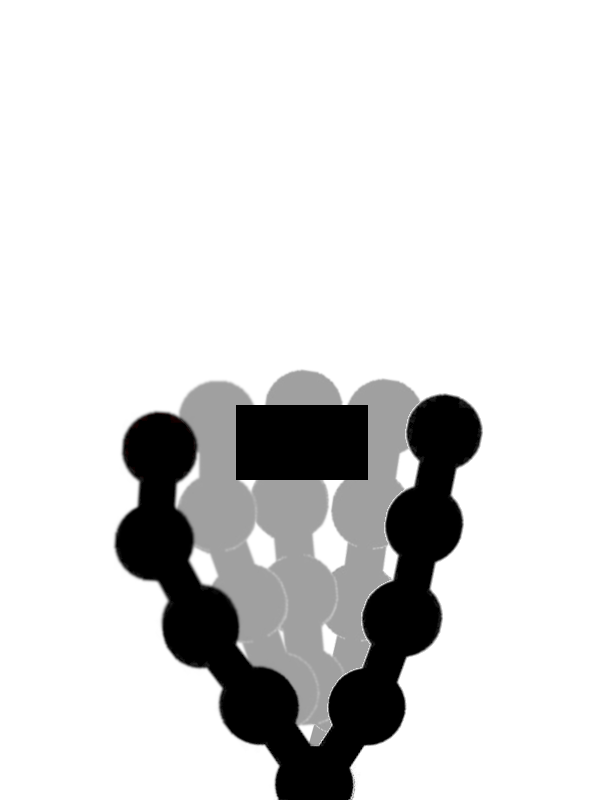
\includegraphics{IK_collision.png}
  \caption{Trying to rotate the joints would lead to a collision with the obstacle}
\end{subfigure}
\caption{A simple case where inverse kinematics is not enough to solve the motion planning problem.}\label{fig:ikcoll}
\end{figure}

\newpage
\section{The RoFI platform}

As technology progresses, research in robotics has moved on from single purpose manipulators used in factories. As of now, we are aiming towards more universal robots; robots that can be deployed in various situations, switch between different tasks, or even change shape. One of the interesting areas from the last few decades has been the concept of modular robots. Modular robots are small independent units, each with their own processors, batteries and usually a few joints. Each module can only perform basic tasks, but they have the ability to connect to each other and build more complex robots. Such a system is not as efficient at performing a single task as a single purpose industrial robot would be, but it has the potential to assemble different robots based on the task at hand and fulfill various roles.


\begin{figure}
    \centering
    
\includegraphics[width=1\textwidth]{rofi_platform.jpg}
  \caption{Logo of the RoFI platform~\cite{rofiPlatform}}
\end{figure}

There have been many research projects concerned with modular robots, each with their own approach to the task at hand. Some projects, such as Roombots~\cite{sprowitz_roombots_2010}, try to build solid structures that can disassemble once their task has been fulfilled. Roombots use sphere shaped modules along with passive blocks to assemble various pieces of furniture, which can be useful for saving space in small apartments or aiding people with disabilities with their daily tasks. Other systems, such as M-TRAN~\cite{mtran} or SMORES~\cite{smores}, try to build mobile robots from more universal modules. Such modules have a joint or two and can perform simple motion; by connecting to each other, they can build bigger robots and fulfill more complex tasks. The designs vary, and there hasn't been any clear winner in the field. An overview on the state of modular robotics can be found here~\cite{modular_survey}, but the field keeps evolving.

The RoFI platform~\cite{Mrázek2019thesis} is an open source modular robotics project developed at Masaryk University. The project is driven by students and consists of algorithmic research~\cite{Vozárová2019thesis, Zacek2021thesis, Nausova2022thesis, Ondika2021thesis, SMTReconfig}, development of hardware~\cite{Mrázek2019thesis, RoFICoM}, networking~\cite{Chlup2020thesis, Chlup2023thesis} and creating tooling for the development of the robots~\cite{Naušová2019thesis, Svoboda2020thesis}.

A robot within this platform, which we refer to as RoFIbot, is comprised of various modules. These can connect and disconnect based on the robot's needs, and allow it to change its overall shape.

\begin{wrapfigure}{r}{0.3\textwidth}
    \centering
    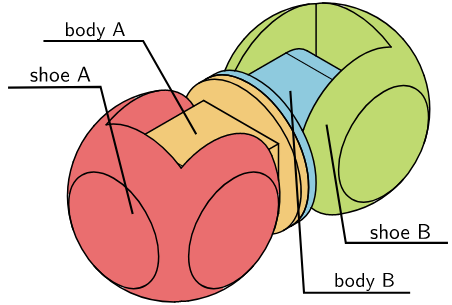
\includegraphics[width=0.3\textwidth]{um.png}
  \caption{Build of the universal module~\cite{rofiUm}}\label{fig:um}
\end{wrapfigure}

The basic building block of each robot within the platform is the universal module. It consists of two symmetrical bodies, wrapped in what we call shoes (see~\ref{fig:um}). The middle part of each module contains the hardware necessary for each module to function as an independent robot in itself. This includes rechargeable batteries to power the whole system, the main processor, which can run user programs, as well as coprocessors that manage firmware. The two bodies are connected to the main unit and perform motion and connection to the other modules.

\begin{wrapfigure}{l}{0.3\textwidth}
    \centering
    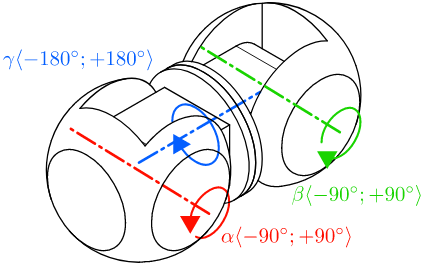
\includegraphics[width=0.3\textwidth]{um_joints.png}
  \caption{Rotation axes~\cite{rofiUm}}\label{fig:um_rot}
\end{wrapfigure}

Each body has a stepper motor that can turn from $-90$ to $90$ degrees. In our models, we refer to the joints as $\alpha$ and $\beta$. Per DH convention, the rotation is calculated as rotation around the $X$ axis with respect to the module's frame. What separates the design of RoFI modules from previous projects such as M-TRAN is the $\gamma$ joint, which allows unlimited rotation around the middle part of the robot, i.e.\ the $Z$ axis. The existence of this joint means that in combination with one of the other motors, the module can perform rotation in any direction, allowing it to perform more complex motions compared to its predecessors.

\begin{wrapfigure}{r}{0.3\textwidth}
    \centering
    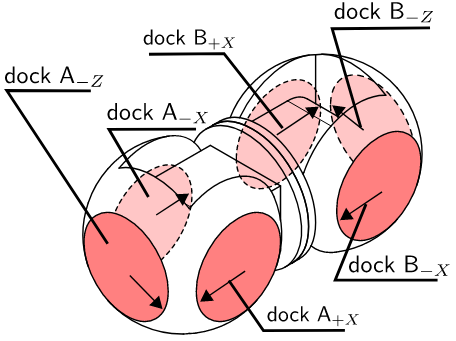
\includegraphics[width=0.3\textwidth]{um_connectors.png}
  \caption{RoFI connectors~\cite{rofiUm}}\label{fig:um_con}
\end{wrapfigure}

Each shoe has 3 connectors; we identify them via the shoe they're on and the direction they're facing with respect to the body. The connectors are genderless, which allows them to connect with any other connector within the plaform, and they can be retracted when not in use. Each connector is equipped with simple Lidar~\cite{Lidar} sensors. These perodically send out a laser that gets reflected off of nearby objects; this allows them to detect obstacles and estimate their distance based on how quickly the reflection returned. As a result, the modules don't have a full view of their environment, but each can locally detect nearby obstacles, as well as recognize whether there is another module they can connect to next to them.

Since each module has 3 degrees of freedom and the modules can be connected in various ways, the DoF of a RoFIbot rises very quickly with each module. If we wish to compute motion for the robot as a whole, traditional algorithms\footnote{Which are generally exponential with respect to the DoF, see the next chapter\ref{SotA}.} quickly become computationally infeasible. As one of the goals for this thesis is control of robotic arms comprised of such modules, a simulation within the RoFI platform will be used to demostrate our results.

  \chapter{State of the art}\label{SotA}

Tady:

- Motion planning as a whole, tj.\ začít s 2D robotem a vysvětlit obecné koncepty, abych se k tomu mohl vracet -- grafové algoritmy, APF, RRT.

- Generalizace A*, APF a RRT na robotická ramena, reference na aktuální články.

- Metody specifické pro robotická ramena, tj.\ hlavně optimalizační.

- Existující pokusy zkombinovat IK a motion planning, tj.\ podobné tomu co dělám já.

% This ensures that the subsequent sections are being included as root
% items in the bookmark structure of your PDF reader.
\bookmarksetup{startatroot}
\backmatter

  \begingroup
    \let\clearpage\relax
    \glsaddall
    \printglossary[type=\acronymtype]
    \newpage
    \printglossary
  \endgroup

  \printindex
  \printbibliography

\end{document}
